\papersubsection{Multi-process abstractions}
\label{sec:eval:pal:multi-proc}

This section evaluates the performance of two multi-process abstractions in \thehostabi:
process creation and bulk IPC.



\paragraph{Process creation.}
Process creation is a relatively expensive
operation in
either one of the PAL implementation.
Instead of adopting copy-on-write style, fork-like semantics,
\thehostabi{} 
only creates clean processes
to avoid the requirement of page sharing.
Therefore, the latency of creating a process,
on either the Linux or \sgx{} PAL,
includes the cost of initializing the PAL binary in a new process or enclave.
The following benchmarks evaluate
the slowdown of process creation in \thehostabi{}
compared with
process creation on a Linux kernel
using \syscall{vfork} and \syscall{execve}.
For accuracy,
the benchmarks measure
the wall time from creating a new process
to receiving the exit notification of the process.
The binary being loaded by \syscall{execve} is a statically compiled program
which returns immediately.


\begin{figure*}[t!]
\centering
\footnotesize
\resizebox{\textwidth}{!}{%
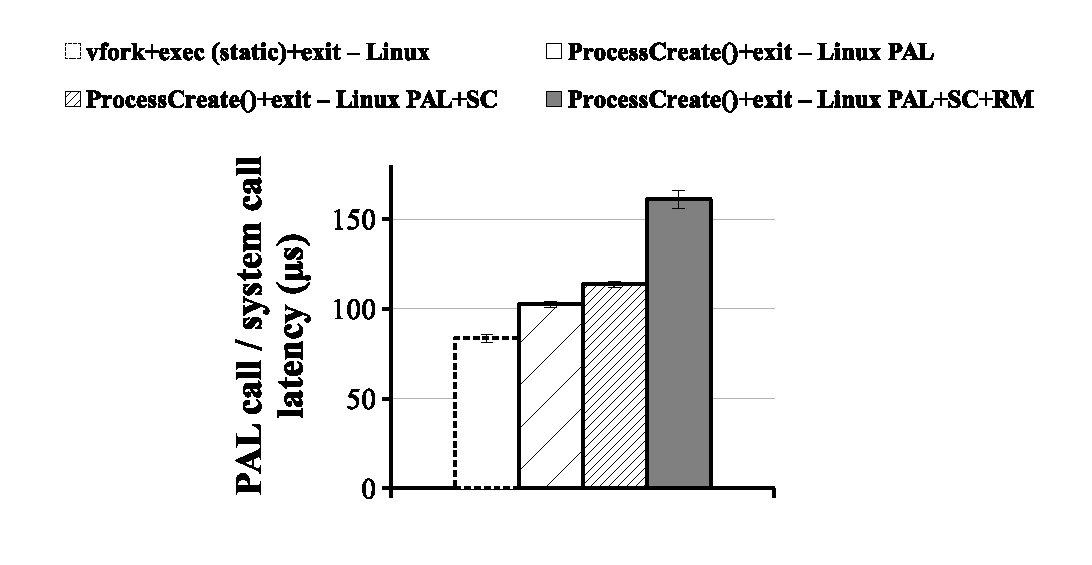
\includegraphics[height=10em]{proc-latency}
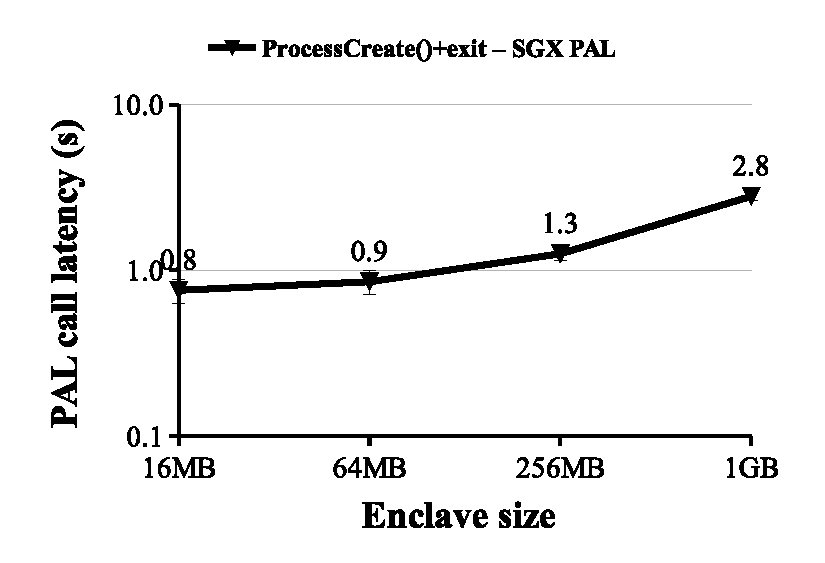
\includegraphics[height=10em]{sgx-proc-latency}
}
\parbox{0.59\textwidth}{\centering\bf (a) process creation+exit}
\parbox{0.39\textwidth}{\centering\bf (b) \sgx{} enclave creation+termination}
\caption{Latency of creating (a) a clean process on the Linux PAL, and (b) an enclave on the \sgx{} PAL, in respect of different enclave sizes.
The comparison is between (1) a combination of \syscall{vfork} and \syscall{exec}'ing a minimal static program on Linux; (2) \palcall{ProcessCreate} on the Linux PAL, with and without a \seccomp{} filter ({\bf +SC}) and reference monitor ({\bf +RM}); (3) the same \hostapi{} on the \sgx{} PAL.}
\label{fig:eval:pal:proc-latency}
\end{figure*}



According to the results shown in
Figure~\ref{fig:eval:pal:proc-latency} (a),
the latency of process creation and exit
on the Linux PAL
is \roughly{}22\% slower than
the latency of similar operations
on a Linux kernel.
The initialization time of the Linux PAL
contributes a large portion to this overhead, besides the minor cost of establishing the RPC stream
between the parent and child processes (using an unnamed UNIX domain socket).
The Linux PAL
with the \seccomp{} filter installed
subjects to the same overheads,
except in order to force the PAL binary always loaded
at the same address,
a separate security loader starts
in each new process
at a low, static address
to load the PAL binary afterwards. 
The overhead with the \seccomp{} filter installed
is \roughly{}26\%,
including the system call slowdown
and the extra cost of reloading the PAL loader in each new process.
If the reference monitor
is enabled,
the reference monitor
must attach the new process to the sandbox
inside the Linux kernel,
and always check that the new process only loads the security loader instead of any other binaries.
The overhead with both the \seccomp{} filter
and the reference monitor
is \roughly{}93\%.



For the \sgx{} PAL,
the latency of creating a new enclave for each child process
is significantly higher
than creating a normal \picoproc{}.
Figure~\ref{fig:eval:pal:proc-latency} (b)
shows that the latency of enclave creation
is related, but not proportional,
to the enclave size configured by users.
To create a 16MB enclave,
which is the minimum size to load a functioning \graphene{} process,
takes \roughly{}0.8\asec{}.
If the enclave size is set at 1GB, the creation time can be up to \roughly{}2.8\asec{},
and will cause significant slowdown
to the guest if the guest frequently spawns processes.
Although some techniques such as
preallocating empty enclave may reduce
the enclave creation time,
this thesis leaves such experiment as future work.
Furthermore,
the \sgx{} version 2 hardware
with support dynamic memory management,
and eliminate the need of preserving large heap space in enclave






 








\begin{figure*}[t!]
\centering
\footnotesize
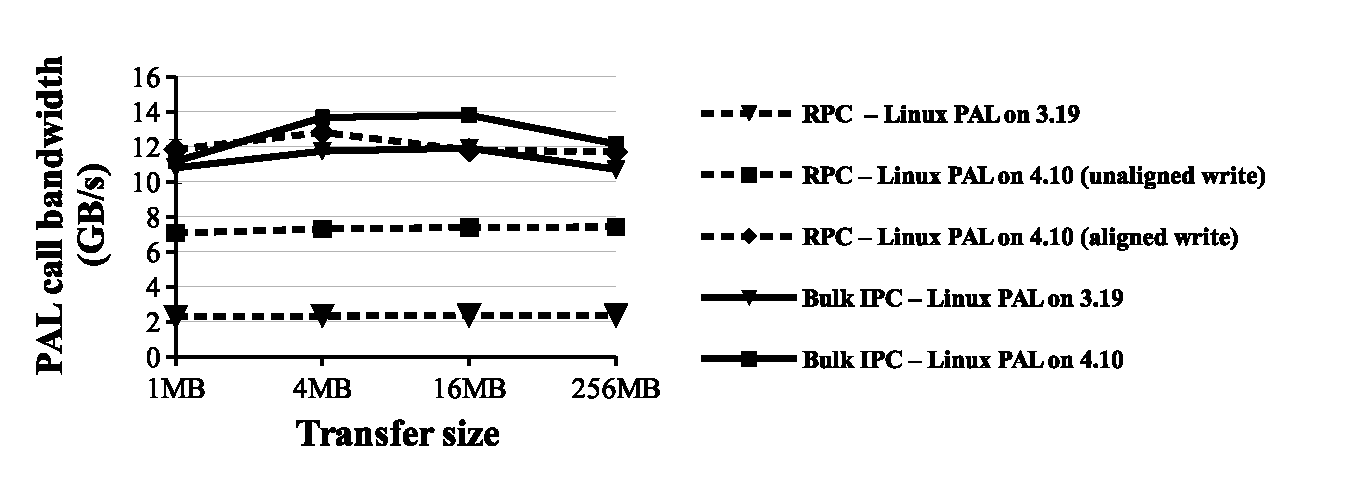
\includegraphics[width=.85\textwidth]{gipc-bandwidth}
\caption{Bandwidth of sending large messages over (a) RPC streams and (b) Bulk IPC channels. The messages are sent in different sizes (1MB to 256MB), and either aligned or unaligned with the page boundary.
Higher is better. Both abstractions are benchmarked on Linux kernel 3.19 and 4.10 as the hosts. The impact of the \seccomp{} filter or reference monitor is marginal (less than 1\%).}
\label{fig:eval:pal:gipc-bandwidth}
\end{figure*}


\paragraph{Bulk IPC vs RPC streams.}
\Thehostabi{} introduces a bulk IPC feature to improve the communication between processes.
Bulk IPC
is an optional feature,
and is assumed to have significantly higher bandwidth
than a regular RPC stream
by sharing the pages as copy-on-write
in another process.
The evaluation results
in Figure~\ref{fig:eval:pal:gipc-bandwidth}
show that
the benefit of using bulk IPC over a RPC stream
subjects to different
host Linux kernel versions.
On a Linux kernel earlier than 4.2, such as the 3.19 kernel evaluated in Figure~\ref{fig:eval:pal:gipc-bandwidth},
the RPC stream
has much lower bandwidth (rough{}32\%) than Linux kernel 4.10.
The reason of the slowdown
is due to the introduction of a zero-copy design of UNIX domain sockets in 4.2.
The zero-copy design
allows a UNIX domain socket to share the physical pages
of a page-aligned buffer
with the destination process,
creating the same effect as the bulk IPC feature in \thehostabi{}.
Therefore, using the bulk IPC is only beneficial on a Linux kernel older than 4.2.






 




